\documentclass[12pt]{article}
\usepackage[utf8]{inputenc}
\usepackage{amsmath}
\usepackage{graphicx}

\title{Latex Tutorials}
\author{Anuj Singh}
\date{February 2020}

\begin{document}

\maketitle  %\to make title
\section{Introduction}
you can write maths inline with text like that $2+3=5$
%\line space will create new paragraph
%\ \\will create new line

superscript example $x^3$

subscript example $x_2$

\section{Geek letters}
$\alpha$
$\beta$
$\gamma$
$\delta$
$\epsilon$

\section{Basic Maths Function}
Here are some basic math functions 

$\sin{x}$

$\sqrt{y}$

$\frac{3}{4}$

\section{Equtions}
\begin{equation}
    x^5+7x^3-4x+2=0
\end{equation}
\begin{equation}
    \sum_{n=1}^{10}\log{n}
\end{equation}
\begin{equation}
    \int_{2}^{3} x^2 dx
\end{equation}
\begin{figure}[!]
    \centering
   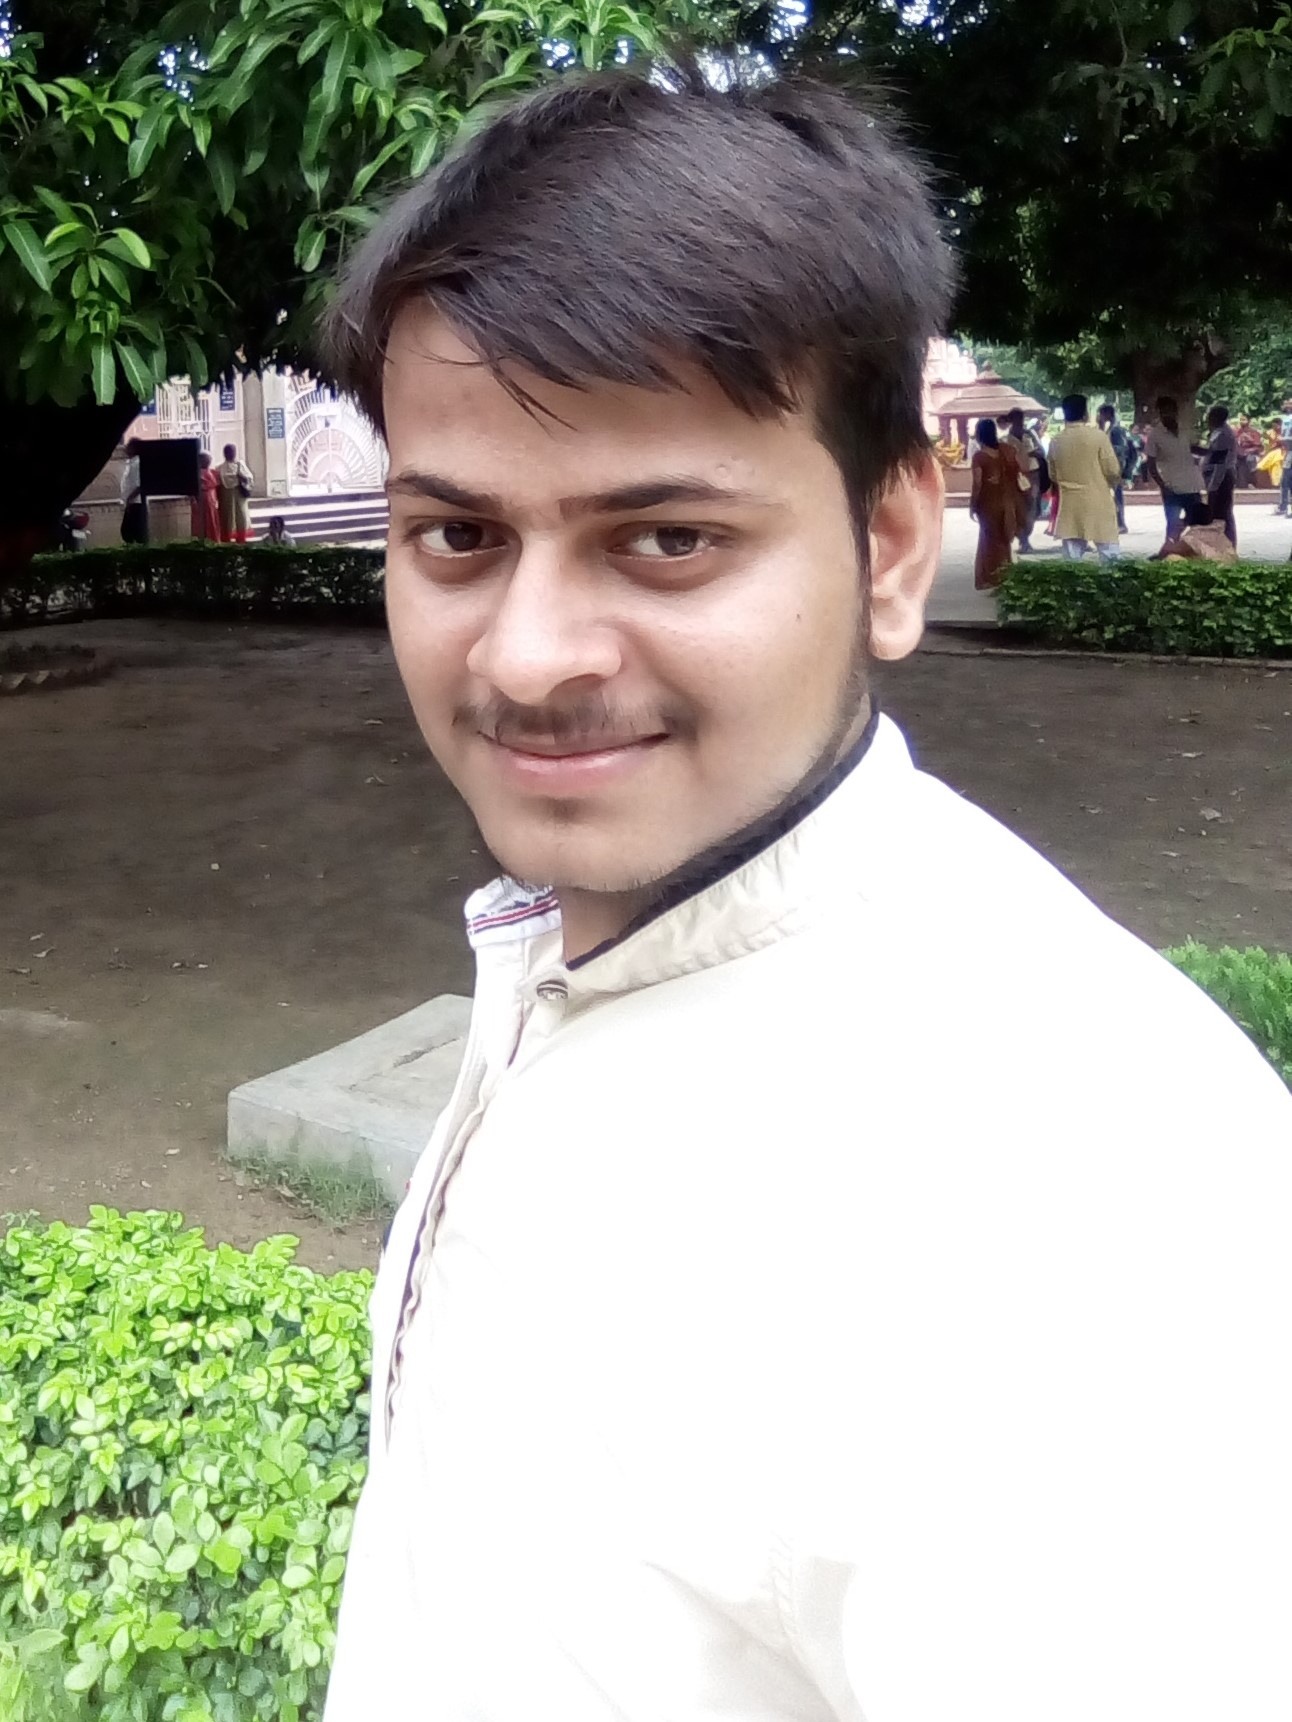
\includegraphics[width=50mm,scale=0.5]{anuj}
    \caption{Anuj Singh}
    \label{fig:anuj}
\end{figure}

see figure \ref{fig:anuj} on page \pageref{fig:anuj}
\section{Table}
\begin{tabular}{l|c|l}
  ID & Name & Branch  \\
  \hline \hline
  20174030 & Anuj & CSE\\
  20179002 & Yogen & Chemical
\end{tabular}}
\section{Matrices}
Here is a Matrix
\[
\begin{matrix}
1 & 2 & 3\\
4 & 5 & 6\\
7 & 8 & 9
\end{matrix}
\]
\[
\begin{pmatrix}
1 & 2 & 3\\
4 & 5 & 6\\
7 & 8 & 9
\end{pmatrix}
\]

\end{document}
